\chapter{Projective Geometry}
\label{chap:projgeo}

\section{The Projective Space}

\subsection{Constructing the Projective Plane}

\subsection{Projective Spaces}

\begin{definition}
  Let $E$ be a finite dimwnsional vector space. The \textit{projective space} $P(E)$ deduced
  from $E$ is the set of all $1$ dimensional linear subspaces of $E$. \cite{audin}
\end{definition}

\begin{remark}
  The dimension of $P(E)$ is $dim$ $E-1$. If $E$ consists only of the point $0$, it does not
  contain any lines, and $P(E)$ is empty. Thus it shall be implicitly assumed that dim $E\ge1$.
  If dim $E=1$, $E$ itself is a line, and thus the set of linea comtains a unique element,
  $P(E)$ is a point.
\end{remark}

\subsection{Projective Subspaces}
A subset $V$ of $P(E)$ is a projective subspace if it is an image of a nonzero vector subspace
$F$ of $E$.

\begin{prop}
  Let $V$ and $W$ be two projective subspaces of $P(E)$.
  
  \begin{itemize}
    \item If dim $V$ + dim $W$ $\ge$ dim $P(E)$, then $V\cap U$ is not empty.
    \item Let $H$ be a hyperplane of $P(E)$, and let $m$ be a point not in $H$. Every
      line through $m$ intersects $H$ at a unique point.
  \end{itemize}

\end{prop}

\begin{proof}
  Let $F$ and $G$ be the vector subspaces of $E$ from which $V$ and $W$ were deduced, i.e.
  $V=P(F)$, and $W=P(G)$. The statement can be translated into vector subspaces as

  \begin{eqnarray*}
    & (\text{dim }F-1)+(\text{dim }G-1)\ge(\text{dim }E-1)\\
    \Longrightarrow& \text{dim }F+\text{dim }G\ge\text{dim }E+1
  \end{eqnarray*}

  We can use the linear algebraic properties to further deduce that:
  \[
    \text{dim }F+\text{dim }G=\text{dim }(F+G)+\text{dim }(F\cap G)
    \le\text{dim }E+\text{dim }(F\cap G)
  \]
  Therefore,
  \[
    \text{dim }(F\cap G)\ge1
  \]
  This can be translated back into projective geometry to conclude that $V\cap W$ is not empty.

  Now, to prove the second property, let $J$ be the vector hyperplane of which $H$ is image of.
  The point $m$ is the image of a line $l$ in $E$, not contained in the hyperplane $J$.
  The assertion, translated in terms of linear algebra, is that any plane $P$ containing $l$
  meets $J$ along a unique line. Since $l$ is not in $J$, we have $P+J=E$. Hence,

  \begin{eqnarray*}
    \text{dim }(P\cap J) &=& \text{dim }P+\text{dim }J-\text{dim }(P+J)\\
    &=& 2+\text{dim }E-1-\text{dim }E=1
  \end{eqnarray*}
\end{proof}

\subsection{Projective Transformations}

\begin{definition}
  Let $E$ and $E'$ be two vector subspaces, and $p:E-\{0\}\rightarrow P(E)$ and
  $p':E'-\{0\}\rightarrow P(E')$ be the two projections. A \textit{projective transformation}
  $g:P(E)\rightarrow P(E')$ is a mapping such that there exists a linear isomorphism
  $f:E\rightarrow E'$ with $p'\circ f=g\circ p$.
\end{definition}

\begin{prop}
  The set of projective transformations from $P(E)$ to itself, $PGL(E)$, is a group under
  composition.
\end{prop}

\begin{proof}
  From the definitions, the projective transformation that descends from identity map of $E$
  forms the identity of the group. For any projective tranformation $g$ that descends from a
  linear isomorphism $f$, the transformation $g'$ that descends from $f^{-1}$ will act as its
  inverse. Since functional composition obeys associativity, $PGL(E)$ is a group.
\end{proof}

\subsection{Homogeneous Coordinates and Projective Frames}

Given a basis of vector space $E$, the vectors in $E$ can be descirbed by their coordinates with
respect to the basis. 

\begin{definition}
  A point $m$ in $P(E)$ can be described by the nonzero vector that generates the line $m$. In a
  n-dimensional projective space $P(E)$, the $(n+1)$ tuples $[x_1,\ldots,x_{n+1}]$ and
  $[x'_1,\ldots,x'_{n+1}]$ represent the same point iff there exists a nonzero scalar $\lambda$
  such that $x_i=\lambda x'_i$ for all $i$.
\end{definition}

In a projective space $P(E)$ with dimension $n$, we actually need $n+2$ points to uniquely determine
the basis of the underlying space $E$, which will be proved in the next lemma. It will also
justify the next definition.

\begin{definition}
  If $E$ is a vector space of dimension $n+1$, a \textit{projective frame} of $P(E)$ is a set of
  $n+2$ points  $(m_0,\ldots,m_{n+1})$ such that $m_1,\ldots,m_{n+1}$ are the images of the
  vectors $e_1,\ldots,e_{n+1}$ in a basis of $E$, and $m_0$ is the image of
  $e_1+\cdots+e_{n+1}$.
\end{definition}

\begin{lemma}
  Let $(m_0,\ldots,m_{n+1})$ be a projective frame of $P(E)$. If the two bases of $E$
  $(e_1,\ldots,e_{n+1})$ and $(e'_1,\ldots,e'_{n+1})$ are such that $p(e_i)=p(e'_i)=m_i$ and
  $p(e_1+\cdots+e_{n+1})=p(e'_1+\cdots+e'_{n+1})=m_0$, then they are proportional.
\end{lemma}

\begin{proof}
  Consider the points $m_i$ of $P(E)$. Since the vectors $e_i$ and $e'_i$ both generate the line
  $m_i$, $e_i=\lambda_i e'_i$ for some nonzero $\lambda_i$. Using the $(n+2)-th$ point, we can
  conclude that 
  \[
    (e_1+\cdots+e_{n+1})=\lambda(e'_1+\cdots+e'_{n+1})
  \]
  Thus,
  \[
    \lambda_1e_1+\cdots+\lambda_{n+1}e_{n+1}=\lambda(e_1+\cdots+e_{n+1})
  \]
  As we are dealing with a basis, $\lambda_i=\lambda$. Thus two bases are proportional.
\end{proof}

\begin{prop}
  Let $P(E)$ and $P(E')$ be two projective spaces of dimension $n$. Any projectivve mapping from
  $P(E)$ to $P(E')$ maps a projective frame of $P(E)$ onto a projective frame of $P(E')$.
\end{prop}

\section{Fundamental Theorem of Projective Geometry}

\begin{theorem}[Fundamental Theorem of Projective Geometry]
  \label{thm:fundprojgeo}
  Let $(a_1,\ldots,a_{n+2})$ and $(b_1,\ldots,b_{n+2})$ be two sets of points in $\R\Ps^n$ such
  that none of the $a_i$ and $b_i$ belong to the projective subspace defined by $n$ of the others
  in their respective sets. Then there exists a unique projective transformation
  $f:\R\Ps^n\rightarrow\R\Ps^n$ such that, $f(a_i)=b_i$ for all $i=1,\ldots,n+2$.
\end{theorem}

\begin{proof}
  The set of points $(a_i)$ and $(b_i)$ are both projective frames of $\R\Pr^n$. Let
  $(e_1,\ldots,e_{n+1}),(e'_1,\ldots,e'_{n+1})\in\R^{n+1}$ be the basis that generate the frames
  $(a_i)$ and $(b_i)$ respectively. We know that there exists a unique isomorphism
  $f:\R^{n+1}\rightarrow\R^{n+1}$ such that $f(e_i)=e'_i$. The projective transformation $g$
  that descends from $f$ will map the first frame to the second.

  To prove the uniqueness: let $f$ and $f'$ two such projcetive transformations. The projective
  transormation $g^{-1}\circ g'$ from $\R\Pr^n$ into itself keeps the frame invariant. Thus
  it is the identity transformation.
\end{proof}

\begin{theorem}[Desargues's Theorem]
  Let $\triangle ABC$ and $\triangle A'B'C'$ be triangles in $\R^2$ such that the lines $AA'$,
  $BB'$, and $CC'$ meet at point $U$. Let $BC$ and $B'C'$ meet at $P$, $CA$ and $C'A'$ at $Q$,
  and $AB$ and $A'B'$ at $R$. Then $P$, $Q$, and $R$ are colinear.
\end{theorem}

\begin{figure}[H]
  \center
  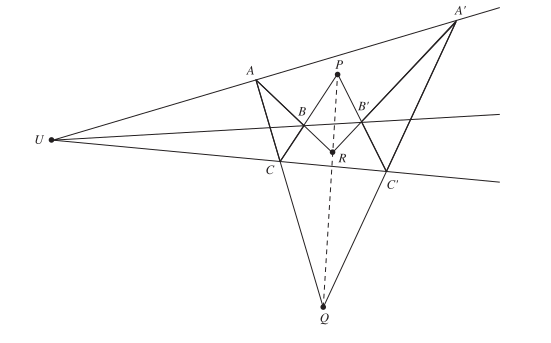
\includegraphics[width=0.75\linewidth]{pictures/desargues.png}
  \caption{Figure from \cite{brannan}.}
\end{figure}

\begin{proof}
  We will prove the theorem for the special case where $A=[1:0:0]$, $B=[0:1:0]$, $C=[0:0:1]$,
  and $U=[1:1:1]$. From the fundamental theorem of projective geometry, we know that it will be
  congruent to any other configuration. We can use the fact that projective congruence preserves
  projrctive properties, to deduce that the theorem holds in general.

  The line $AU$ has the equation $y=z$. Since $A'$ lies on $AU$, it must have coordinates
  $[a:b:b]$, where $b\ne 0$, since $A'\ne A$. We can also wirte $A'=[p:1:1]$, where $p=a/b$.
  Similary, $B'=[1:q:1]$, and $C'=[1:1:r]$.

  Now to find the point $P$, we find the equation of the line $BC$.
  \[
    \begin{vmatrix}
      x & y & z\\
      1 & q & 1\\
      1 & 1 & r
    \end{vmatrix}
    =0\Longrightarrow (qr-1)x-(r-1)y+(1-q)=0
  \]
  Substituting $x=0$ in the equation for the line $B'C'$, we get $(r-1)y=(1-q)z$, which immplies
  $P=[0:1-q:r-1]$. Similarly we find that $Q=[1-p:0:r-1]$, and $R=[1-p:q-1:0]$.

  To check the colinearity of $P$, $Q$, and $R$:
  \[
    \begin{vmatrix}
      0   & 1-q & r-1 \\
      1-p & 0   & r-1\\
      1-p & q-1 & 0
    \end{vmatrix}
  \]
  \begin{eqnarray*}
    &=& -(1-q)(1-p)(1-r)+(r-1)(1-p)(q-1)\\
    &=& 0
  \end{eqnarray*}

  i.e $P$, $Q$, and $R$ are colinear.
\end{proof}

\begin{prop}
  There is a unique projective conic through any given set of five points, no three of which are
  collinear.
\end{prop}

\begin{proof}
 By the fundamental theorem of projective geometry, there exists a projective transformation
 $t$ which maps the four out of given five points to the points $[1:0:0]$, $[0:1:0]$, $[0:0:1]$
 and $[1:1:1]$. Let $[a:b:c]$ be the image of the fifth point under $t$. Since projective
 transformations preserve collinearity, no three of the five points are collinear, and also
 it can be deduced that $a$, $b$ and $c$ are nonzero, since if it were so, it would be collinear
 with other two points.

 Let the conic that passes through these 5 points be of the form
 \[
   Ax^2+Bxy+Cy^2+Fxz+Gyz+Hz^2
 \]
 By substituting the points $[1:0:0]$, $[0:1:0]$, and $[0:0:1]$, the equation can be reduced
 to the form
 \[
   Bxy+Fxz+Gyz=0
 \]
 Since the porjective concic also passes through $[1:1:1]$ and $[a:b:c]$, we get the equations
 \[
   B+F+G=0
 \]
 and
 \[
   Bab+Fac+Gbc=0
 \]
 Solving these simultaneous equations, we get
 \[
   F=-G\frac{ab-bc}{ab-ac}
 \]
 and
 \[
   B= -G\frac{ac-bc}{ac-ab}
 \]
 It follows that the conic is of the form
 \[
   -G\frac{ac-bc}{ac-ab}xy-G\frac{ab-bc}{ab-ac}xz+Gyz=0
 \]
 or
 \[
   c(a-b)xy+b(c-a)xz+a(b-c)yz=0
 \]
 Since the conic is uniquely determined by the fifth point, it follows that it is unique.\\
\end{proof}

\begin{remark}
  \textbf{The Standard Projective Conic}

  The projective conic $E=\{[x:y:z]:xy+yz+zx=0\}$ is called the standard projective conic.
  It passes through the traingle of reference formed by the points $[1:0:0]$, $[0:1:0]$, and
  $[0:0:1]$. This fact can be used to simplify calculations involving projcetive conics.

  All the points on the conic except than $[1:0:0]$ can be parameterized as $[t^2+t:t+1:-t]$,
  where $t\in\R$. All points on $E$ satisfy $xy+yz+zx=0$. Suppose $y\ne 0$, let $t=x/y$. Then
  $x=ty$, and so

  \begin{eqnarray*}
    & (ty)y+yz+z(ty)=0 \\
    \Longrightarrow & ty+(t+1)z=0 \\
    \Longrightarrow & y=-\frac{t+1}{t}z, x=-(t+1)z
  \end{eqnarray*}

  Thus the point has homogeneous coordinates $\left[-(t+1)z:-\frac{t+1}{t}z:z\right]$, which can
  be rewritten in the form $[t(t+1):t+1:-t]$. This also happens to hold for the point $[0:0:1]$,
  where $y=0$.
\end{remark}

\begin{prop}
  Let $E_1$ and $E_2$ be non-degenrate conics that pass through the points $P_1$, $Q_1$, $R_1$
  and $P_2$, $Q_2$, $R_2$ respectively. THen ther exists a projective transformation $t$ which
  maps $E_1$ to $E_2$ such that $t(P_1)=P_2$, $t(Q_1)=Q_2$, and $t(R_1)=R_2$.
\end{prop}

\begin{proof}
  We prove this result by proving that for any conic $E_1$, there exists a transormation $t_1$
  which maps it to the standard conic $xy+yz+zx=0$ such that $t_1(P_1)=[1:0:0]$,
  $t_2(Q_1)=[0:1:0]$, and $t_3(R_1)=[0:0:1]$ for any $P_1,Q_1,R_1\in E$.

  Let $f$ be a transformation that maps $P_1$ to $[1:0:0]$, $Q_1$ to $[0:1:0]$, and $R_1$ to
  $[0:0:1]$. It will map the conic $E_1$ into a conic $E'$ of the form
  \[
    Fxy+Gyz+Hzy=0
  \]
  for some $F,G,H\in\R$. Divide the equation by $FGH$ to rewrite $E'$ in the form
  \[
    \frac{xy}{GH}+\frac{yz}{FH}+\frac{zx}{FG}=0
  \]
  Now, let $g$ be the transformation of the form $g([x:y:z])=A[x:y:z]\forall[x:y:z]\in\R\Pr^3$
  where $A$ is a $3\times 3$ matrix such that
  \[
    A=
    \left(\begin{array}{ccc}
      \frac{1}{H} & 0           & 0           \\
      0           & \frac{1}{G} & 0           \\
      0           & 0           & \frac{1}{F} \\
    \end{array}\right)
  \]
  Then, $g$ maps $E'$ to the standrd conic $xy+yz+zx=0$, leaving $P$, $Q$, and $R$ unchanged.
  Let $t_1=g\circ f$. Similarly, let $t_2$ be the function that maps the conic $E_2$ to the
  standard conic such that $t_2(P_2)=[1:0:0]$, $t_2(Q_2)=[0:1:0]$, and $t_2(R_2)=[0:0:1]$
  for any $P_2,Q_2,R_2\in E_2$.

  The composite function $t=t_2^{-1}\circ t_1$ maps $E_1$ to $E_2$ such that $t(P_1)=P_2$,
  $t(Q_1)=Q_2$, and $t(R_1)=R_2$, as required.
\end{proof}

\begin{theorem}[Pascal's Theorem]
  Let $A$, $B$, $C$, $A'$, $B'$, and $C'$ be six distinct points on a non-degenrate projective
  conic. Let $BC$ and $B'C$ intersect at $P$, $CA'$ and $C'A$ at $Q$, and $AB'$ at $R$. The
  points $P$, $Q$, and $R$ are collinear.
\end{theorem}

\begin{figure}[H]
  \center
  
\includegraphics[width=\linewidth]{pictures/pascal.png}
  \caption{Figure from \cite{brannan}.}
  \label{fig:pascal}
\end{figure}

\begin{proof}
  We know that any non-degenerate conic can pe transformed to the standard conic. Let the conic
  be in the standard form $xy+yz+zx=0$, with $A=[1:0:0]$, $B=[0:1:0]$, and $C=[0:0:1]$. Let the
  point $A'=[a^2+a:a+1:-a]$, $B'=[b^2+b:b+1:-b]$, and $C'=[c^2+c:c+1:-c]$, for some $a,b,c\in\R$

  The line $BC'$ has the equation $x=-(c+1)z$, and the line $B'C$ has the equation $x=by$. The
  point $P$ lies on both of these lines. Hence it has the homogeneous coordinates
  $[b(c+1):c+1:-b]$. Similarly, $Q=[a(c+1):c+1:-c]$, and $R=[b(a+1):b+1:-b]$.

  To check their collinearity, evaluate the determinant:
  \[
    \begin{vmatrix}
      b(c+1) & c+1 & -b \\
      a(c+1) & c+1 & -c \\
      b(a+1) & b+1 & -b \\
    \end{vmatrix}
  \]
  Which, after some row operations, simplifies to be equal to $0$.
  Hence, the points $P$, $Q$, and $R$ are collinear.
\end{proof}

Proof adapted from \cite{brannan}.

\section{The Cross-Ratio}

\begin{definition}
  Let $a$, $b$, $c$ and $d$ be four points on a projective line $D$. There exists a unique map
  from $D$ to $K\cup\{\infty\}$ that maps $a$ to $\infty$, $b$ to $0$, and $c$ to $1$. The
  image of $d$ under this projective mapping is called the \textit{cross-ratio} of the points
  $(a,b,c,d)$, and denoted $[a,b,c,d]$.
\end{definition}

\begin{prop}
  Let $a_1$, $a_2$, $a_3$, and $a_4$ be four points on the line $D$ (the first three being
  distinct) and $a'_1$, $a'_2$, $a'_3$, and $a'_4$ be four points on another line $D'$
  (satisfying the same assumption). There exists a projective transformation $f:D\rightarrow D'$
  such that $f(a_i)=a'_i$ iff $[a_1,a_2,a_3,a_4]=[a'_1,a'_2,a'_3,a'_4]$.
\end{prop}

\begin{proof}
  Assume $f$ is a projective mapping that sends $a_i$ to $a'_i$. Let $g$ and $g'$ be functions
  such that $[a_1,a_2,a_3,a_4]=g(a_4)$, and $[a'_1,a'_2,a'_3,a'_4]=g'(a'_4)$. $g'\circ f$ is a
  function, which maps $a_1$ to $\infty$, $a_2$ to $0$, and $a_3$ to $1$. But such function is
  unique. Hence, $g=g'\circ f$, which implies that $g(a_4)=g'(a'_4)$. That is,
  \[
    [a_1,a_2,a_3,a_4]=[a'_1,a'_2,a'_3,a'_4]
  \]
\end{proof}

\section{Elliptic Curves}

\begin{definition}
  An elliptic curve is a non-empty, non-singular, degree 3 projective curve. \cite{spallone}
\end{definition}

\subsection{Group Laws on Conics}
